\section{Versuchsauswertung}

\subsection{Kalibrierung}

\subsubsection{Fixpunktkalibrations an der Wassertripelpunktzelle}

Zunächst wurde der Pt-100 (Vierleiterschaltung) Referenzsensor anhand der Wassertripelzelle (Tripelpunkt bei \SI{0,01}{\celsius} und \SI{6,1}{\milli\bar}) mittels Fixpunktkalibration kalibriert. In der folgenden Abbildung \ref{fig:Fixpunkt} wird der Temperaturverlauf in Abhängigkeit der Zeit (die Scanrate beträgt \SI{1}{\sec}) für den Pt-100 Sensor abgebildet. 

\begin{figure}[H]
	\centering
	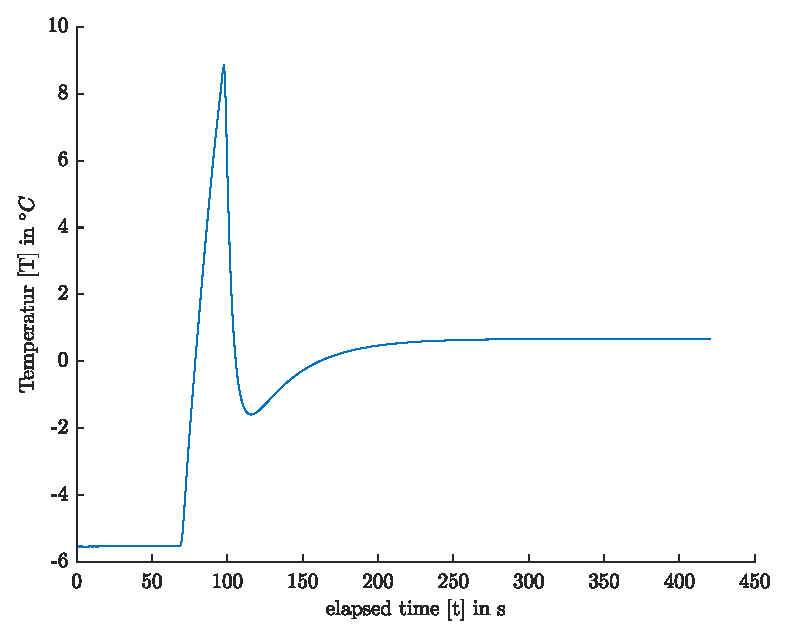
\includegraphics[height=0.3\textheight]{../MLAB/Fixpunktkalibration.eps}
	\caption[Temperaturverlauf des Pt100 Temperatursensors mittels Wassertripelpunktzelle]{ Temperaturverlauf des Pt100 Temperatursensors mittels Wassertripelpunktzelle im Metallblockkalibrator.}
	\label{fig:Fixpunkt}
\end{figure}

Folgende Daten wurden für den Mittelwert, die Standardabweichung und den Offset des Referenzsensors gegenüber der Temperatur der Tripelpunktzelle ermittelt: 


\begin{table}[H]
	\centering
	\caption{Mittelwert, Standardabweichung und Offset des Pt100 4L Referenzsensors zur Tripelpunktzelle.}
	\label{tab:VergleichTPZ}
	\begin{tabular}{c|c|c|c}
		Temperatur TP [\si{\celsius}] & avg & std & Offset \\ 
		\hline 
		\num{0.01} & \num{0.6691} & \num{0.0024} &  \num{0.6591}\\ 
	\end{tabular} 
\end{table}


Im folgenden wurden mit dem ermittelten Offset des Referenzsensors dessen Messwert korrigiert und bei den folgenden Berechnungen berücksichtigt und angepasst. 

\subsubsection{Vergleichskalibration der Sensoren}

Die Vergleichskalibration der unterschiedlichen Sensoren erfolgte in einem Temperaturbereich von \SI{0}{\celsius} bis \SI{80}{\celsius}, für die Messungen wurden über den Pt100 4L die Temperaturen \SI{0}{\celsius}, \SI{20}{\celsius}, \SI{40}{\celsius} und \SI{80}{\celsius} ausgewählt und über den Metallblockkalibrator eingestellt. In der folgenden Abbildung \ref{fig:Widerstand} sind die Widerstände der einzelnen Temperatursensoren gegen die ausgewählten Temperaturmesspunkt aufgetragen. 

\begin{figure}[H]
	\centering
	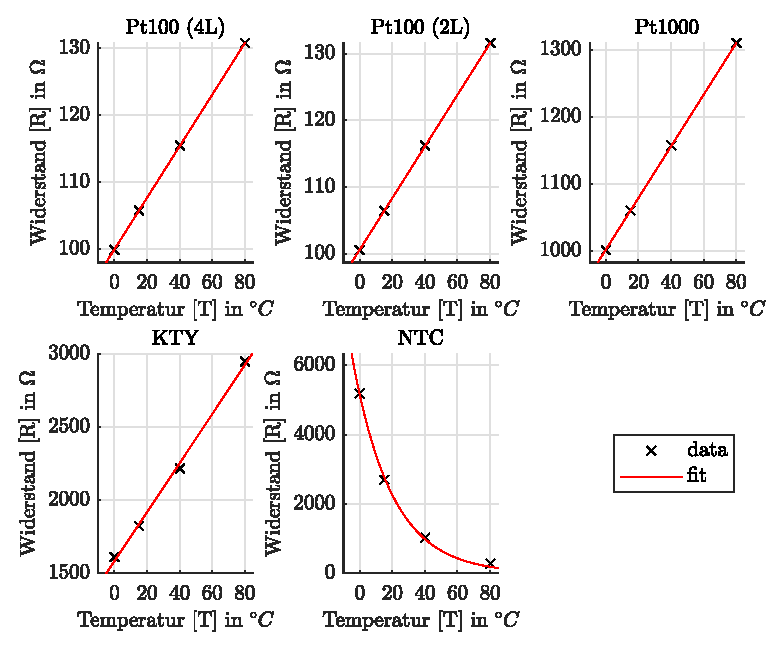
\includegraphics[height=0.5\textheight]{../MLAB/Widerstandsgeraden.eps}
	\caption[Ermittelte Widerstandswerte der untersuchten Temperatursensoren ]{Ermittelte Widerstandswerte der untersuchten Temperatursensoren (Pt100 4L, Pt100 2L, Pt1000, KTY, NTC bei den Temperturen \SI{0}{\celsius}, \SI{20}{\celsius}, \SI{40}{\celsius} und \SI{80}{\celsius} im Metallblockkalibrator eingestellt über den Pt100 4L Referenzsensor. }
	\label{fig:Widerstand}
\end{figure}

Die Temperatursensoren Pt100 4L, Pt100 2L, Pt1000 und KTC zeigen lineare Widerstandsverläufe positiver Steigung bei Erhöhung der Temperatur. Das Kaltleiter-Thermometer (NTC-negative temperature coeffizient) zeigt aufgrund seines negativen Temperaturkoeffizienten ein exponentiell abfallendes Verhalten. 

\subsubsection{Vergleich von Pt100 4L und Pt100 2L}

Bei der Messung wurden unter anderem ein Pt100 in Vierleiterschaltung und ein Pt100 in Zweileiterschaltung verwendet. Die beiden Thermometer unterscheiden sich in ihrer Anschlussart. Bei Widerstandsthermometern wird die Messgenauigkeit durch den Leitungswiderstand der Kabel stark beeinflusst wird (dieser wird mit zunehmender Kabellänge größer). Bei einem Pt 100 der Klasse B können bei 
\begin{figure}[H]
	\centering
	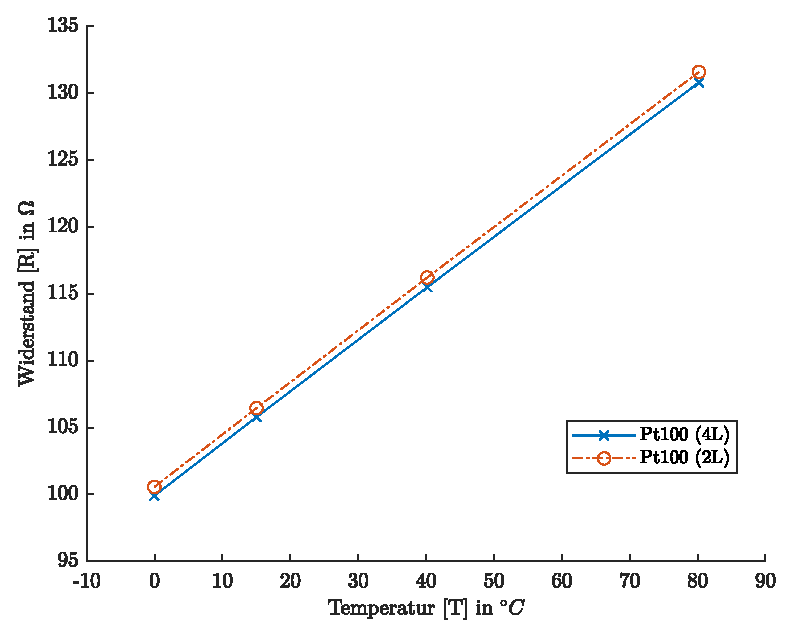
\includegraphics[height=0.3\textheight]{../MLAB/Vergleich2L4L.eps}
	\caption[Temperaturverlauf des Pt100 Temperatursensors mittels Wassertripelpunktzelle]{ Temperaturverlauf des Pt100 Temperatursensors mittels Wassertripelpunktzelle im Metallblockkalibrator.}
	\label{fig:2L4L}
\end{figure}
